\documentclass{beamer}
%\usetheme[numbering=none,nofirafonts]{gitcourse}
\usetheme{metropolis}

\definecolor{main}{RGB}{92, 138, 168}
\definecolor{background}{RGB}{240, 247, 255}

\usepackage{sourcecodepro}
%\usepackage[osf]{mathpazo}

\usepackage{booktabs}
\usepackage{amsmath}
\usepackage{amssymb}
\usepackage{amsfonts}
\usepackage{amsthm}
\usepackage{mathdots}
\usepackage{mathtools}
\usepackage{cancel}
\usepackage{braket}
\usepackage{listings}

\newcommand{\git}{Git{}}
\newcommand{\cd}[1]{\texttt{#1}}

\title{\git, GitHub and GitFlow}
\author{Jacopo Schiavon}
\institute[Dep. Statistical Sciences --- UNIPD]{Department of Statistical Sciences\\ University of Padova}


\begin{document}
\begin{frame}[plain]
    \maketitle
\end{frame}

\begin{frame}{}
\tableofcontents
\end{frame}

\section{Introduction to \git}
\begin{frame}{What is \git?}
    \alert{\git} is a \alert{free} and \alert{open source} distributed \alert{version control system} (VCS) designed to handle everything from small to very large projects with speed and efficiency. 
    
    Its goals include \alert{speed}, \alert{data integrity}, and support for \alert{distributed} and \alert{non-linear} workflows.
    
    \begin{block}{History of \git}
        \begin{itemize}
            \item Created in 2005 by Linus Torvald (now maintained by Junio Hamano)
            \item Its original purpose was helping developing the Linux kernel
            \item It is designated for coordinating the work of many developer on the same project
            \item It is very useful also for smaller projects
        \end{itemize}
    \end{block}
\end{frame}

\begin{frame}{Why \git?}
    \git{} is used to manage projects consisting of \alert{text files}: \cd{R} or \cd{Python} packages and scripts; \LaTeX{} documents; repositories of text files (\textit{i.e.} configs for servers or desktops).
    
    Its most advanced features are useful when cooperating in a team of developers.
    \begin{block}{Why \git{} for small project?}
        \begin{itemize}
            \item It teaches \alert{good practices} in code developing and maintaining
            \item It greatly simplify \alert{versioning} 
            \item It rationalize the management of new or experimental features
            \item Combined with GitHub, it trivialize \alert{code sharing}
            \item It helps with keeping track of the \alert{history of the code}.
        \end{itemize}
    \end{block}
\end{frame}

\begin{frame}{\git{} features}
    \begin{itemize}
        \item \alert{Branching} \git{} main feature, will have an entirely dedicated slide.
        \item \alert{Small and Fast} All \git{} procedures (and \git{} itself) are fast and minimal: one or two commands to do everything. Committing and pushing requires no more than a couple of seconds $\Rightarrow$ almost no impact on the workflow.
        \item \alert{Entire history of the repository} \git{} keeps all versions of all files that it is tracking. Allows you to check differences between every two versions (or reverting to any version) of your code.
        \item \alert{Distribution} \git{} structure implies that each developer works on its own (\textit{forked}) version of a central repository, without breaking or interfering with the work of others developers.
        \item \alert{Cryptographic assurance} Every bit that \git{} tracks is authenticated by advanced cryptographic techniques.
    \end{itemize}
\end{frame}

\begin{frame}{\git{} features: Branching}
    \begin{itemize}
    \item Main idea: possibility to \alert{work in parallel} on the same code. 
    \item Useful also when working alone: possibility of \alert{testing different features} without creating copies. 
    \item A \alert{branch} is a new line of history of the code, completely independent from the rest
    \item \git{} allows to \alert{create}, \alert{switch} and \alert{merge} different branches with minimal effort (one command for each operation).
    \end{itemize}

    \begin{figure}
        \centering
        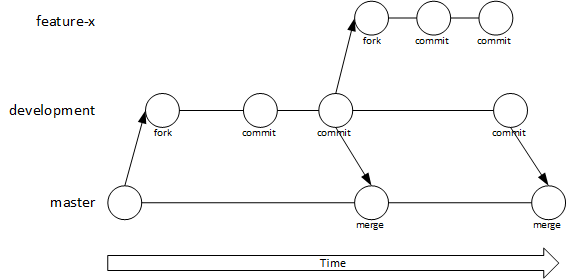
\includegraphics[width=0.7\textwidth]{git_workflow_1.png}
    \end{figure}
\end{frame}

\begin{frame}{\git{} features: Branching}
    \begin{block}{Examples of use cases for small projects}
        \begin{itemize}
            \item Try a different implementation of a function not knowing if it will work better
            \item Try to rewrite a paragraph or chapter, not knowing if it will come out better
            \item Keep version of a document in another language
            \item Test a new functionality that might break another part of the code
        \end{itemize}
    \end{block}
\end{frame}

\begin{frame}{How to use it in practice? [UNIX systems]}
    UNIX systems are mainly MacOS or GNU/Linux (but also FreeBSD). Usually \git{} is already installed in your system
    \begin{block}{To create a \git{} repository:}
        \begin{itemize}
            \item Create the folder that you want to track with \git{} (or use one already in use)
            \item Open a terminal emulator and move to the location of the folder
            \item Give the command \cd{git init}
            \item You are ready to start committing!
        \end{itemize}
    \end{block}
\end{frame}

\begin{frame}{How to use it in practice? [Windows]}
    Usually \git{} is not installed. 
    \begin{itemize}
        \item Download the windows installer from \url{https://git-scm.com/} and execute it.
        \item Follow the procedure for installation, installing the Git Bash.
        \item Now, clicking with the right button on a folder will allow you to open a Git Bash window, which will work exactly as a UNIX terminal.
    \end{itemize}
    
\end{frame}

\section{Introduction to GitHub}
\begin{frame}{Frame Title}
\end{frame}

\section{Introduction to GitFlow}
\begin{frame}{Frame Title}
\end{frame}

\section{Some useful commands}
\begin{frame}{Local file management}
\begin{table}
    \scriptsize
    \centering
    \begin{tabular}{p{0.4\textwidth}p{0.5\textwidth}}
        \toprule
        \alert{Command}	&	\alert{Meaning}\\
        \midrule
        \texttt{git init}	&	Initiate a local repository in the folder\\
        \texttt{git status}	&	Shows the status of the file in the repository (new, modified, already stashed)\\
        \texttt{git add [\textit{file}]}	&	Add \texttt{\textit{file}} to the staging area\\
        \texttt{git commit -m "\textit{msg}"} & Record a permanent snapshot of the staged files with an associated message \textit{msg}\\
        \texttt{git log}	&	Shows the history of commits for the current branch\\
        \texttt{git log -{}-pretty=oneline}	&	Shows a compressed version of the log\\
        \texttt{git diff}	&	Shows not yet staged differences\\
        \bottomrule
    \end{tabular}
\end{table}
\end{frame}

\begin{frame}{Branching}
\begin{table}
    \scriptsize
    \centering
    \begin{tabular}{p{0.4\textwidth}p{0.5\textwidth}}
        \toprule
        \alert{Command}	&	\alert{Meaning}\\
        \midrule
        \texttt{git branch}	&	List all branches\\
        \texttt{git branch [\textit{name}]}	&	Create a branch named \textit{name}\\
        \texttt{git checkout [\textit{name}]}	&	Switch to the branch named \textit{name}\\
        \texttt{git merge [\textit{name}]}	&	Combines the branch named \textit{name} with the current branch\\
        \bottomrule
        \end{tabular}
    \end{table}
\end{frame}

\begin{frame}{Online repository}
\begin{table}
    \scriptsize
    \centering
    \begin{tabular}{p{0.4\textwidth}p{0.5\textwidth}}
        \toprule
        \alert{Command}	&	\alert{Meaning}\\
        \midrule
        \texttt{git clone \textit{url}}	&	Download an online repository to your local filesystem\\
        \texttt{git pull}	&	Download and integrate the online changes to the repository\\
        \texttt{git fetch}	&	Download all the remote repository history\\
        \texttt{git push [\textit{alias}] [\textit{branch}]}	& Pushes the local commits in the current branch to the \textit{branch} of online repository named \textit{alias}\\
        \bottomrule
        \end{tabular}
\end{table}
\end{frame}

\end{document}


